\section{Fundamentals of Particle Image Velocimetry}

Particle Image Velocimetry, or PIV, is a class of methods employed by 
experimental fluid mechanics to measure instantaneous vector velocity fields by 
measuring the displacements of small visible particles which follow the motion 
of the fluid \cite{adrian2011}. Figure \ref{fig:quiver_example} shows a typical 
resulting vector field from measurements of a vortical flow. Each of these 
two-dimensional vectors was measured simultaneously in a thin sheet of fluid. 
The velocity of the fluid is sensed by acquiring images of well entrained 
particles at precise times and measuring the displacement of those particles. 
This is accomplished with the use of cameras for acquiring images and an 
intense laser to illuminate particles within the desired plane. 
This technique can be used to study flows in gases and liquids, and is derived 
from techniques originally developed to measure deformations on the surface of 
solid material.

\begin{figure}[H]
	\centering
	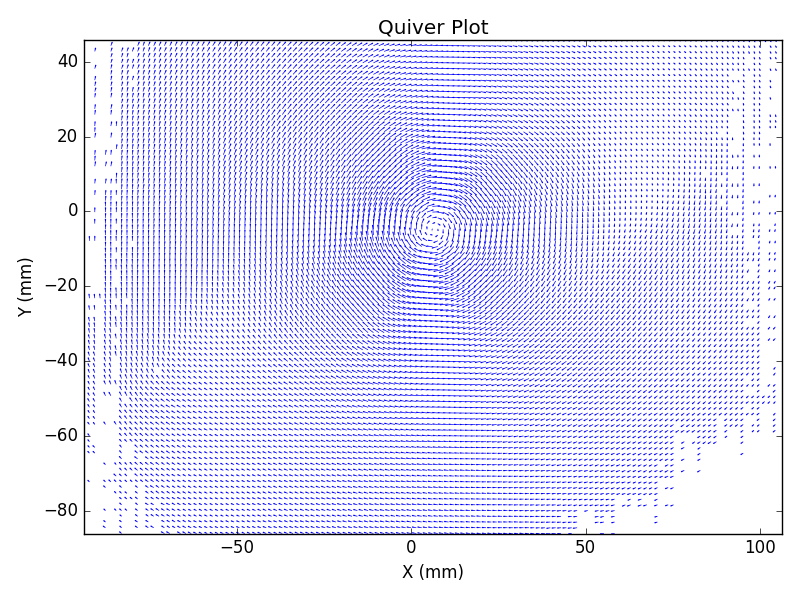
\includegraphics[width=5in]{figs/example_vortex_figs/example_quiver}
	\caption{Velocity vector field of a vortical flow structure as produced by 
	PIV.}
	\label{fig:quiver_example}
\end{figure}

 
\subsection{The Case for PIV}

Unlike other flow measurement techniques, PIV is a non-invasive method to 
directly measure time and displacement, and thus velocity. PIV is also capable 
of resolving vector measurements at many positions within a two dimensional 
slice of the flow field simultaneously, while other measurement techniques 
require taking data at many locations sequentially over a much greater period 
of time. Single camera PIV can measure two components of the velocity vectors 
aligned with the image plane, but the PIV method is capable of resolving many 
dimensions of fluid flow with incremental increases in system complexity. The 
addition of another camera allows the full three dimensional velocity vector to 
be measured, and a sweeping beam laser allows the interrogation of an entire 
volume of flow field instead of a slice.

Stereo PIV is used widely because it provides a full velocity vector, and 
requires only an additional camera, slightly more complex calibration and 
software to process the imagery.  A stereo PIV system with a 
stationary sheet laser can resolve three dimensional velocity vectors and their 
fluctuations within a two dimensional slice of fluid flow. A two point 
correlation tensor containing important information about the turbulent 
structure of a flow can be obtained readily with PIV. The non-invasive nature 
of PIV, combined with the  ability to interrogate a flow volume very quickly 
for information with high dimensionality makes it exceptionally useful in fluid 
mechanics. \cite{adrian1991}

\subsection{Cameras and Lighting}

\subsection{Particles}

\subsubsection{Particle Dynamics} 

\subsubsection{Error Due to Slip}

\subsubsection{Seeding Particles for PIV}

\subsection{Image processing}

\cite{soloff1997, willert1997}.

\subsection{Interrogation}

\subsection{Measurement of Fluid Flow}

\subsection{PIV in Three Dimensions}

\subsection{Practical PIV Systems}


